\chapter{File system forensics domain // Da completare} 

The field of file system forensics is focused on analyzing file systems to retrieve hidden or deleted data. This domain is essential for forensic investigations as it uncovers information about the organization and structure of file storage, even after files have been deleted.

\section{File System Forensics}

Key aspects of file system forensics include:
\begin{itemize}
    \item \textbf{Slack Space Analysis:} Investigating unused portions of disk sectors which may still contain residual data from previously stored files.
    \item \textbf{File Carving:} Recovering deleted files by analyzing data remnants in disk clusters, a method useful when files have been deleted but not overwritten.
    \item \textbf{Registry and Configuration Analysis:} Retrieving user or system activities from OS configurations, such as the Windows Registry or Unix configuration files (e.g., \texttt{/etc}, \texttt{\~/.config}, \texttt{\~/.bashrc}). (this part of the analysis is usually done during the OS forensics)
\end{itemize}

Common tools in this field include low-level utilities like \texttt{stat}, \texttt{istat}, and \texttt{debugfs} as well as high-level software such as FTK Imager and Autopsy.

\section{File System}

A file is the smallest logical unit of storage from the user’s perspective, organized into bytes, lines, or records. File systems are essential for structuring and managing files, with the operating system (OS) mapping logical files to physical storage (e.g., memory addresses, disk sectors, or cloud resources). Through these mappings, file systems define rules for reading, writing, and maintaining data on storage devices.

\section{File Attributes}

Files are typically characterized by the following attributes:
\begin{itemize}
    \item \textbf{Name:} A mnemonic identifier for referencing files. Older systems, like DOS, had an 8+3 character naming format, which modern OS no longer limit.
    \item \textbf{Type:} Indicates the file category, often determined by a \textbf{“magic number}”: few bytes at the start of the file. Windows OS, however, may rely on extensions to associate files with applications, but for analysis is better referring to the magic number. 
    \item \textbf{Protection:} Access control information varies across OS, specifying ownership and permissions (e.g., read, write, execute permissions on Unix systems).
    \item \textbf{Location:} The physical or logical storage location.
    \item \textbf{Size:} Specifies the file’s storage size.
\end{itemize}

\section{File System Formatting}

File system formatting is the process that prepares a mass storage device for data storage by configuring it with specific file system structures. This operation is essential for organizing data storage, defining how files will be written, stored, and accessed on a storage medium.

\begin{itemize}
    \item \textbf{Data Erasure:} Formatting typically erases existing information on the storage device. 
    \begin{itemize}
        \item \textbf{Full Formatting:} This is a slower process that erases all sectors by writing zeros across the storage and identifies any bad sectors, marking them as unusable.
        \item \textbf{Quick Formatting:} A faster alternative that only erases the file system tables, leaving the actual data sectors untouched.
    \end{itemize}
    \item \textbf{Partitioning:} Formatting can create one or more partitions on the storage device. Each partition can function as a separate logical volume, with primary, extended, or logical partitions.
    \item \textbf{File System Selection:} During formatting, a specific file system is selected based on the operating system requirements. Common file systems include:
    \begin{itemize}
        \item \textbf{NTFS} for Windows, \textbf{APFS} for macOS, \textbf{ext4} for Linux.
    \end{itemize}
    \item \textbf{Foundational Structures Creation:} The formatting process also establishes essential file system structures. These structures enable data organization and include:
    \begin{itemize}
        \item Root directory, FAT/Inode table, superblock/Boot sector
    \end{itemize}
\end{itemize}

This formatting process is crucial for initializing a storage device, defining its structure, and ensuring compatibility with the operating system and user requirements.


\subsection{FAT File System Example}

When formatting a hard drive with a FAT file system:
\begin{itemize}
    \item The Boot Record is created, containing information such as the OS name, disk characteristics (as bytes per sectors, sectors per cluster, root directory entry).
    \item The Master File Table (MFT) is established, with two copies for redundancy, detailing clusters' status (available, allocated, damaged, or used by OS files).
    \item A Directory Table organizes the structure of top-level files and directories.
\end{itemize}

The FAT system is noted for its portability and ease of use but lacks advanced features such as encryption and robust access controls, making it less secure.

\begin{figure}[ht]
    \centering
    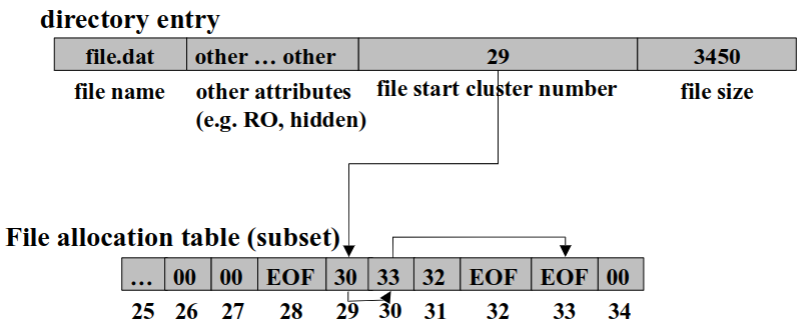
\includegraphics[width=0.8\textwidth]{img/fat.png}
    \caption{Example of a FAT File System Structure}
    \label{fig:fat_file_system}
\end{figure}

\subsubsection{FAT pros and cons}
\begin{itemize}
    \item portability (available to multiple operating systems)
    \item migration (easy switch to richer FS, like NTFS)
    \item fast on small volumes (some GB), due to light "infrastructure (few metadata, no file index, ...)
    \item no integrated advanced features (on-the-fly compression, user quotas)
    \item slow for high numer of files (linked-list structure, fragmentation, no)
    \item no security at all (encryption, access control lists)
\end{itemize}

\section{File Copy and Cloning}

Simple file copy commands preserve file content but may alter file metadata. For forensics, bit-by-bit copies ensure fidelity to the original data, often using the \texttt{dd} command. Variants of \texttt{dd} (e.g., \texttt{dcfldd} and \texttt{dc3dd}) offer additional features like on-the-fly hashing and pattern wiping.

Example commands:
\begin{itemize}
    \item Clone a hard drive to another: \texttt{dd if=/dev/sda of=/dev/sdb}
    \item Create an image file of a hard drive: \texttt{dd if=/dev/hda of=/image.img}
    \item Wipe a drive with binary zeros: \texttt{dcfldd pattern=00 vf=/dev/hdb}
    \item \dots
\end{itemize}

\section{File Identification}

File identification involves determining a file’s actual type and contents, which is crucial in forensics to verify the authenticity and integrity of data. This process often extends beyond simply looking at file extensions, as these are not a reliable source of information.

\begin{itemize}
    \item \textbf{Limitations of Extensions:} File extensions can be easily altered by users or malicious actors, so they should not be solely relied upon to identify a file type.
    \item \textbf{Metadata Inspection:} Whenever possible, examine the file’s metadata, as it often contains information about the file’s true format and origin.
    \item \textbf{File Signatures:} The first few bytes of a file can act as a unique signature, known as a "magic number," which can confirm the file type. A reference list of file signatures can be found online (e.g., \url{https://en.wikipedia.org/wiki/List_of_file_signatures}).
    \item \textbf{Hex Dump Comparison:} By comparing a file's signature with its hex dump, investigators can verify the file type independently of the extension.
\end{itemize}

\section{Metadata Example: File System}

File systems maintain metadata for each file, providing critical information about its content and history. This metadata, managed by the operating system, includes:

\begin{itemize}
    \item \textbf{File Name, Ownership, and Permissions:} Details about the file’s identity, access rights, and owner.
    \item \textbf{Allocated Data Units:} Information on the specific data blocks or clusters assigned to the file.
    \item \textbf{File Size:} The size of the file in bytes.
    \item \textbf{Timestamps:} Key dates associated with the file, such as creation, modification, and last access times.
    \item \textbf{Recovery Data:} Some file systems maintain recovery information (e.g., journaling) that aids in data recovery processes.
\end{itemize}

The type and accuracy of metadata can vary significantly based on the file system in use. Common file systems with differing metadata structures include FAT32, NTFS, ext2, ext3, and ext4.

\section{Slack Space}

Slack space is residual storage within disk sectors allocated to files but not fully utilized. For example, if a 392-byte file is stored in a 512-byte sector, the remaining 120 bytes become slack space, potentially retaining data from prior file storage.

\section{File Recovery Process}

File recovery in forensics involves analyzing file system structures such as the Master File Table (MFT), which stores file metadata, including timestamps. This enables timeline reconstruction, which is crucial for investigating user actions in legal cases. Deleted files, also known as orphan files, may still be recoverable depending on the level of data overwriting and fragmentation.

\section{Metadata Analysis in Files}

Metadata, or "data about data," provides additional insights into file characteristics. Common examples include EXIF metadata for images or embedded metadata in office documents (e.g., DOCX, ODF). Metadata analysis can reveal hidden information, enhance context, and correlate data across files, though it is not inherently trustworthy and may be modified.

\section{Data Sanitization}

Data sanitization tools permanently erase data to prevent unauthorized recovery. Common methods include:
\begin{itemize}
    \item \textbf{File Shredder Programs:} Permanently overwrite selected files.
    \item \textbf{Data Destruction Software:} Fully erases all data on a storage device, useful for secure disposal or virus removal.
\end{itemize}

The Air Force System Security Instruction (AFSSI) 5020 specifies a three-pass overwrite process to ensure data irretrievability.

